% =============================================================================
% SAMBP: Three-Phase Differential Protection Model Diagram
% File: differential_protection_model.tex
% Description: Block diagram showing current decomposition and model parameters
% =============================================================================

\documentclass[tikz,border=10pt]{standalone}
\usepackage{tikz}
\usepackage{amsmath}
\usetikzlibrary{shapes,shapes.geometric,arrows,arrows.meta,calc,positioning,fit,decorations.pathmorphing}

\begin{document}

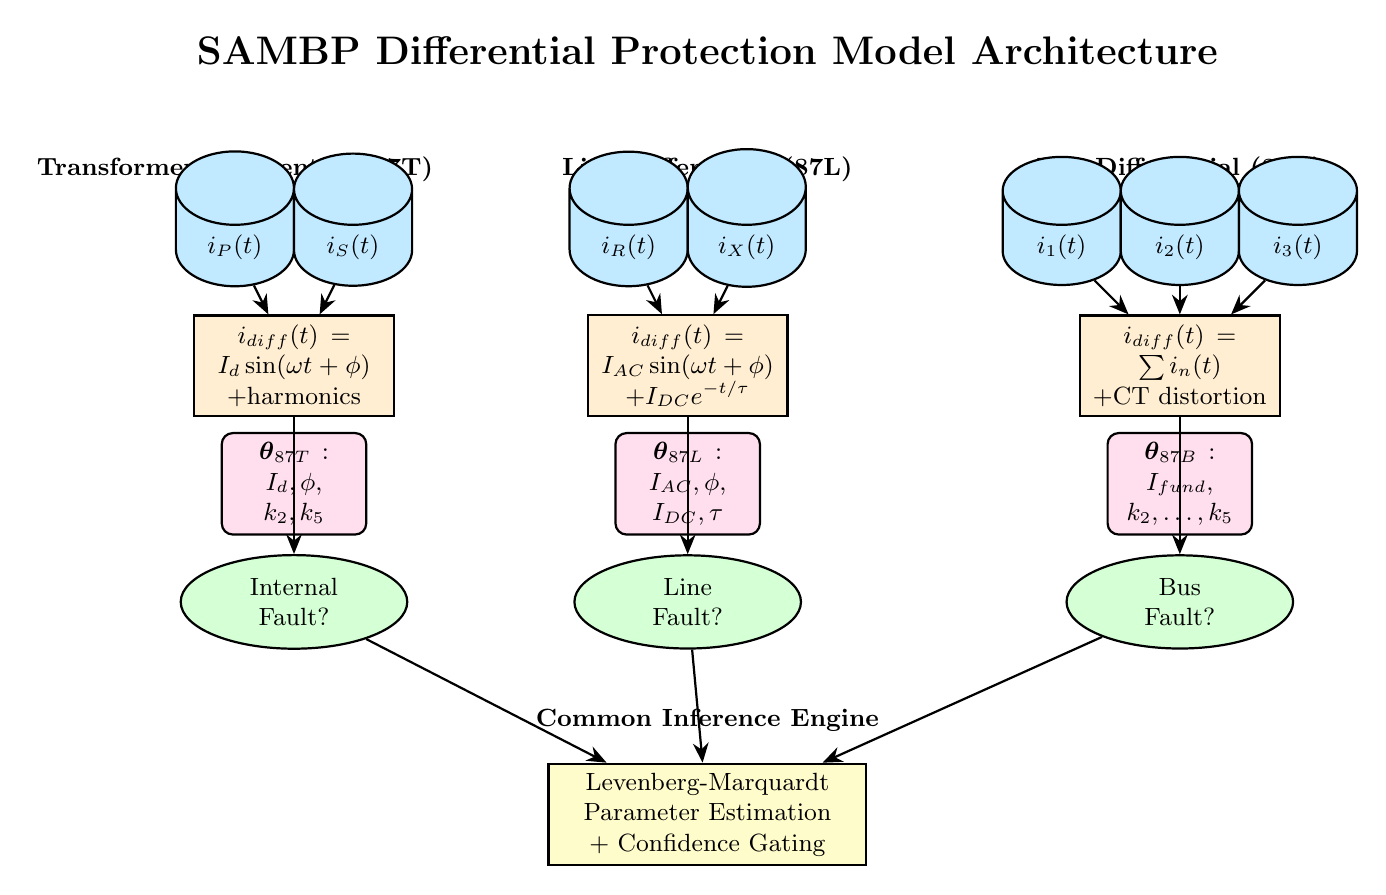
\begin{tikzpicture}[
    node distance=1.5cm,
    font=\small,
    >=latex,
]

\definecolor{inputCol}{RGB}{100, 200, 255}
\definecolor{modelCol}{RGB}{255, 200, 100}
\definecolor{outputCol}{RGB}{150, 255, 150}
\definecolor{paramCol}{RGB}{255, 150, 200}

\tikzset{
    input_node/.style = {cylinder, shape border rotate=90, minimum width=1.5cm, minimum height=0.8cm,
                         text centered, draw=black, thick, fill=inputCol!40},
    model_node/.style = {rectangle, minimum width=2.5cm, minimum height=0.8cm,
                         text centered, text width=2.3cm, draw=black, thick, fill=modelCol!30},
    output_node/.style = {ellipse, minimum width=2cm, minimum height=0.8cm,
                          text centered, text width=1.8cm, draw=black, thick, fill=outputCol!40},
    param_node/.style = {rectangle, rounded corners, minimum width=1.8cm, minimum height=0.7cm,
                         text centered, text width=1.6cm, draw=black, thick, fill=paramCol!30},
    arrow/.style = {thick, -{Stealth[length=2.5mm, width=2mm]}},
    label/.style = {font=\scriptsize, inner sep=2pt}
}

% Title
\node at (6, 9) {\Large \textbf{SAMBP Differential Protection Model Architecture}};

% =========== TRANSFORMER DIFFERENTIAL (87T) ===========
\node at (0, 7.5) {\textbf{Transformer Differential (87T)}};

\node[input_node] (i_p) at (0, 6.5) {$i_P(t)$};
\node[input_node] (i_s) at (1.5, 6.5) {$i_S(t)$};

\node[model_node] (87t_model) at (0.75, 5) {\small $i_{diff}(t) =$\\$I_{d}\sin(\omega t+\phi)$\\$+\text{harmonics}$};

\node[param_node] (87t_theta) at (0.75, 3.5) {$\boldsymbol{\theta}_{87T}:$\\ $I_d, \phi$,\\ $k_2, k_5$};

\node[output_node] (87t_out) at (0.75, 2) {Internal\\Fault?};

% Arrows for 87T
\draw[arrow] (i_p) -- (87t_model);
\draw[arrow] (i_s) -- (87t_model);
\draw[arrow] (87t_model) -- (87t_out);
\draw [thick, dashed] (87t_theta) -- (87t_model);

% =========== LINE DIFFERENTIAL (87L) ===========
\node at (6, 7.5) {\textbf{Line Differential (87L)}};

\node[input_node] (i_r) at (5, 6.5) {$i_R(t)$};
\node[input_node] (i_x) at (6.5, 6.5) {$i_X(t)$};

\node[model_node] (87l_model) at (5.75, 5) {\small $i_{diff}(t) =$\\$I_{AC}\sin(\omega t+\phi)$\\$+I_{DC}e^{-t/\tau}$};

\node[param_node] (87l_theta) at (5.75, 3.5) {$\boldsymbol{\theta}_{87L}:$\\ $I_{AC}, \phi$,\\ $I_{DC}, \tau$};

\node[output_node] (87l_out) at (5.75, 2) {Line\\Fault?};

% Arrows for 87L
\draw[arrow] (i_r) -- (87l_model);
\draw[arrow] (i_x) -- (87l_model);
\draw[arrow] (87l_model) -- (87l_out);
\draw [thick, dashed] (87l_theta) -- (87l_model);

% =========== BUS DIFFERENTIAL (87B) ===========
\node at (12, 7.5) {\textbf{Bus Differential (87B)}};

\node[input_node] (i_1) at (10.5, 6.5) {$i_1(t)$};
\node[input_node] (i_2) at (12, 6.5) {$i_2(t)$};
\node[input_node] (i_3) at (13.5, 6.5) {$i_3(t)$};

\node[model_node] (87b_model) at (12, 5) {\small $i_{diff}(t) =$\\$\sum i_n(t)$\\$+\text{CT distortion}$};

\node[param_node] (87b_theta) at (12, 3.5) {$\boldsymbol{\theta}_{87B}:$\\ $I_{fund}$,\\ $k_2, \ldots, k_5$};

\node[output_node] (87b_out) at (12, 2) {Bus\\Fault?};

% Arrows for 87B
\draw[arrow] (i_1) -- (87b_model);
\draw[arrow] (i_2) -- (87b_model);
\draw[arrow] (i_3) -- (87b_model);
\draw[arrow] (87b_model) -- (87b_out);
\draw [thick, dashed] (87b_theta) -- (87b_model);

% =========== COMMON INFERENCE ENGINE ===========
\node at (6, 0.5) {\textbf{Common Inference Engine}};

\node[rectangle, minimum width=4cm, minimum height=0.8cm, text centered,
      text width=3.8cm, draw=black, thick, fill=yellow!20] (lm_engine) at (6, -0.7) {
    Levenberg-Marquardt Parameter Estimation + Confidence Gating
};

\draw[arrow] (87t_out) -- (lm_engine);
\draw[arrow] (87l_out) -- (lm_engine);
\draw[arrow] (87b_out) -- (lm_engine);

\end{tikzpicture}

\end{document}
